\documentclass[a4page, 11pt]{article}

\usepackage{graphicx}
\usepackage{mathtools}
\usepackage[margin=1.2in]{geometry}
\usepackage[utf8]{inputenc}
\usepackage[italian]{babel}
\usepackage{enumitem}

\graphicspath{ {./img/} }
\title{\textbf{Social Issues in Information Society}}
\author{}
\date{}


\begin{document}
\maketitle


\section*{Lezione 1 - 05/11/2018}
(Dall'introduzione di \textit{The Game}, Alessandro Baricco, Einaudi, 2018). \newline
Gli umani sembrano aver disimparato tutto ciò che avevano imparato dai loro padri, come mangiare, studiare, divertirsi.
Un particolare sconcerto si ha nella osservazione quotidiana dei figli: a Baricco sembrano tornare indietro nel miglioramento della specie, incapaci di concentrarsi, sempre attaccati a qualche computer.
Si intuiva l'annuncio di qualche crisi e l'imminenza di una apocalisse culturale.
La faccenda non era chiarissima, sicuramente c'entravano la rivoluzione digitale e la globalizzazione.
Altri umani, perlopiù in California, stavano cambiando il mondo tecnicamente, senza spiegare al resto dell'umanità il loro progetto, se ne avevano uno, e forse senza manco sapere quali conseguenze avrebbe avuto tutto ciò.
Ma come mai abbiamo accettato l'idea di una rivoluzione?
Ora abbiamo tante cose che vent'anni fa non esistevano: Wikipedia, Facebook, YouTube\ldots{} che occupano una buona parte del nostro tempo, così tanto che ci chiediamo come facevamo 20 anni fa a trascorrere le giornate.
È un mondo che non saperemo mai spiegare, è una rivoluzione di cui non sappiamo né l'origine, né lo scopo.
Baricco sente l'emozione della paura nei confronti di tale rivoluzione. \newline

I biologi classificano gli esseri viventi in specie: a una specie appartengono quelli esseri che possano riprodursi.
Le specie che hanno un antenato in comune e che si sono evolute in modo diverso sono raggruppate in \textit{generi}.
Noi siamo del genere \textit{homo} specie \textit{sapiens}.
I generi a loro volte solo raggruppati in \textit{famiglie}.
Noi ci siamo evoluti dagli \textit{australopitecus}, da cui è uscito l'uomo di Neanderthal più muscolosi del \textit{sapiens}.
Da 2.5 milioni a circa 10 mila anni fa, il pianeta è stato occupato da diverse specie di homo; negli ultimi 10 mila anni l'uomo è salito sulla vetta della piramide alimentare, grazie al suo cervello più sviluppato.
Circa 70 mila anni fa l'uomo di Neanderthal si è diffuso dall'Africa Orientale in Medio Oriente, e poi in tutto il mondo.
Ci sono due teorie per spiegare la loro scomparsa:
\begin{itemize}
  \item Teoria della fusione (l'uomo moderno è l'unione di più specie);
  \item	Teoria del rimpiazzo (i \textit{sapiens} hanno rimpiazzato le altre specie di ominidi).
\end{itemize}
La teoria più accreditata è quella del rimpiazzo: i \textit{sapiens} erano più efficaci come cacciatori, avevano una organizzazione sociale migliore ed erano più avanzati tecnologicamente rispetto ai Neanderthal.
È il primo caso di genocidio mai registrato: i \textit{sapiens} hanno spazzato via tutti i Neanderthal.
Di grande aiuto può essere stata l'invenzione del linguaggio e del pensiero astratto, permesse dall'evoluzione della specie: queste realizzazioni hanno portato a una rivoluzione cognitiva dei \textit{sapiens} che introduce nuove capacità:
\begin{itemize}
  \item permette di trasmettere più volumi di informazione, riuscendo a pianificare azioni più complesse, come cacciare animali feroci;
  \item inventare nuovi oggetti utili;
  \item trasmettere maggiori volumi di informazione circa le relazioni sociali, permettendo la creazione di gruppi più ampi e coesi, fino a 150 persone (i gruppi di Neanderthal invece erano più piccoli quindi è stato facile per i \textit{sapiens} sterminarli);
  \item trasmettere idee più astratte, come gli spiriti tribali, le Nazioni, le responsabilità, i diritti\ldots e questo ebbe come conseguenze:
  \begin{itemize}
    \item una cooperazione tra un numero molto alto di estranei grazi alle credenze comuni;
    \item una rapida innovazione del comportamento sociale.
  \end{itemize}
\end{itemize}
Questo aumento della capacità cognitiva può essere dovuto ad una mutazione genetica, o, secondo un'altra teoria, per permettere i pettegolezzi, teorizzando la natura sociale dell'\textit{homo sapiens}.

I passaggi dalla Preistoria alla Storia e infine all'Iperstoria sono definiti in base al ciclo di vita dell'informazione.
Il ciclo è costruito in questo modo: l'informazione si Genera $\Rightarrow$ Raccoglie $\Rightarrow$ Immagazzina $\Rightarrow$
Elabora $\Rightarrow$ Distribuisce $\Rightarrow$ Consuma $\Rightarrow$ Ricicla $\Rightarrow$ Genera.

Nella Preistoria, parte fondamentalmente ha la rivoluzione agricola, avvenuta circa nel 10 mila A.C.: in questa epoca non ci sono documentate forme di ICT (intendiamo per ICT forme di immagazzinamento o di documentazione), queste compaiono nella Storia (nel 3000-4000 A.C.) ma il benessere non ne è ancora collegato (nel ciclo di vita dell'informazione ci si ferma all'immagazzinamento, l'informazione non si processa).
L'iperstoria invece è dipendente dalle ICT: il benessere sociale e individuale dipende da come si processa e si fa uso delle informazioni.\newline
\begin{center}
  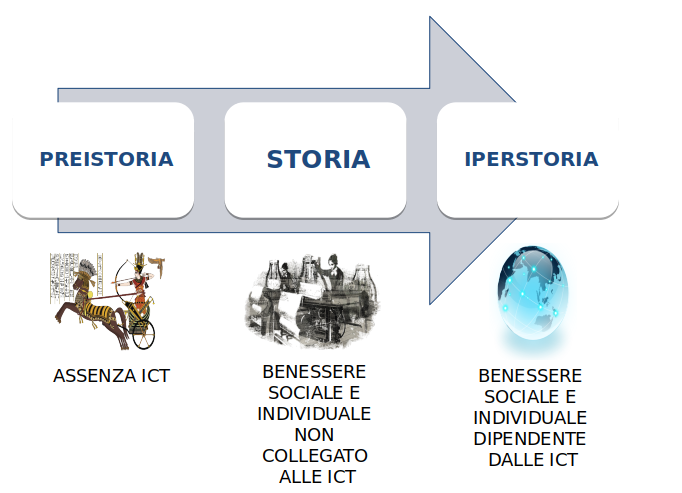
\includegraphics[scale=0.5]{image1.png}
\end{center}

Due tipi principali di rivoluzioni sono:
\begin{itemize}	 
  \item Le rivoluzioni politiche: sono caratterizzata da violenza e rapidità, tra loro collegate; sono cambiamenti traumatici dello stato del mondo o del Paese dovuti a fenomeni radicali a livello politico o economico; questa violenza e rapidità si manifesta nella prima metà del 1900.
  \item Le rivoluzione tecnologiche e scientifiche: di per sè non violente ma hanno delle conseguenze che possono esserlo.
\end{itemize}

Thomas Kuhn sostiene che le rivoluzioni scientifiche mettono in crisi un intero paradigma del mondo e finché il nuovo paradigma non si afferma la rivoluzione scientifica non può passare.
La rivoluzione digitale è in primo luogo una rivoluzione tecnologica.
Le rivoluzioni tecnologiche sono dovute all'invenzione di oggetti o strumenti nuovi che cambiano il modo di vivere mentre le rivoluzioni tecnologiche possono anche essere fantastiche ma di rado producono una rivoluzione mentale.
Una rivoluzione tecnologica può essere \textit{disruptive} sulla società o sull'economia ma diventa una rivoluzione mentale solamente se modifica profondamente il modo di pensare e la scala di valori delle persone; queste vengono anche dette rivoluzione scientifiche.
Le rivoluzione tecnologiche principali sono:
\begin{enumerate}
  \def\labelenumi{\arabic{enumi}.}
  \item rivoluzione dell'agricoltura (circa 10.000 A.C.): è stata una delle rivoluzione più difficili perché ha forzato l'uomo a lavorare di più, ma ha dato le basi al mondo attuale;
  \item rivoluzione industriale (seconda metà del XVII secolo);
  \item rivoluzione dell'informazione (metà del XIX secolo): nascono le tecnologie digitali.
\end{enumerate}
Mentre le rivoluzioni scientifiche principali sono:
\begin{enumerate}
  \def\labelenumi{\arabic{enumi}.}
  \item rivoluzione copernicana: (la Terra non è al centro dell'Universo): ha avuto bisogno di molto tempo prima di riuscire a passare nella società a causa delle implicazioni sociali e religiose che portava con sè;
  \item rivoluzione darwiniana (l'uomo non è al centro del mondo animale): l'uomo non ha un posto privilegiato all'interno del regno animale;
  \item rivoluzione freudiana (la mente umana non è trasparente a se stessa ma è caratterizzata dall'inconscio e dal meccanismo del repressione);
  \item rivoluzione dell'informazione: non siamo entità isolate ma interconnesse, composte da agenti biologici e artefatti tecnici, che popolano un ambiente globale costituito dall'informazione (l'infosfera) che assorbe il mondo reale e lo ingloba in un mondo informatico.
\end{enumerate}
La rivoluzione informatica, basata sul silicio e non più sul carbonio, è quindi non solo rivoluzione tecnologica ma anche scientifica.


\section*{Lezione 2 - 07/11/2018}
Le transazioni da società storica a società iperstorica sono:
\begin{itemize}
  \item Legge di Moore: la tecnologia di un microcircuito raddoppia ogni 18 mesi.
  \item Legge di Metcalfe: se $n$ è il numero di utenti in una rete, il numero massimo di connessione è $\frac{1}{2}n(n-1)$, cioè la crescita del numero di connessioni, e di conseguenza il costo riguardante la tecnologia, è quadratica rispetto al numero di utenti.
  \item Forte crescita dei dispositivi connessi.
  \item Sviluppo sinergico delle nuove tecnologie digitali (Cloud, IoT, Mobile\ldots).
  \item Crescita esponenziale dei \textit{Big Data}, definiti come:.
    \begin{itemize}
      \item Secondo IDC, una nuova generazione di tecnologie e di architetture disegnate per estrarre il valore economico da grandi volumi e varietà di dati, a grande velocità, con complesse operazioni di gestione e di analisi (le $5$ V: Velocità, Volume, Varietà, Variabilità e Veridicità).
      \item Secondo NIST, i Big Data si riferiscono alla difficoltà delle architetture tradizionali a gestire efficacemente i nuovi dataset. Le caratteristiche dei Big Data sono: Volume, Velocità, Varietà e/o Variabilità. I Big Data sfruttano la distribuzione orizzontale e indipendente dei dati per ottenere la potenza di calcolo richiesta per una gestione dei database estensivi. 
    \end{itemize}
\end{itemize}

I Big Data sono diversi dai database tradizionali perché hanno alti Volumi di dati non strutturati e devono essere memorizzati e processati rapidamente: richiedono nuove architetture e nuovi sistemi di elaborazione e di visualizzazione.
Per ottenere questi risultati, i Big Data sfruttano la scalabilità sia in verticale (aumento di potenza), sia in orizzontale con l'utilizzo di risorse distribuite. Sono usati in una serie di ambiti:
\begin{itemize}
  \item identificare clienti a più alto potenziale per la vendita di prodotti collegati ed effettuare pubblicità mirata (ROI\footnote{\textit{Return On Investment}, misura l'efficacia di un investimento. Si calcola come: $ROI = \frac{\text{risultato operativo (della gestione caratteristica)}}{\text{capitale investito netto operativo}}$, ovvero, indicativamente, il ricavato dall'investimento rispetto al valore totale investito.}: 41-56\%);
  \item identificare i bisogni dei clienti (ROI: 40-48\%);
  \item identificare i clienti a rischio e analizzarne il comportamento (ROI: 54\%);
  \item monitorare la qualità e quantità (ottimizzata) dei prodotti necessari (ROI: 50-70\%);
  \item misurare il rischio, pianificare azioni, calcolare budget e altre previsioni (ROI: 69\%);
  \item migliorare la gestione dei dividendi  e l'efficacia del reclutamento (ROI: 48\%).
\end{itemize}

I Big Data hanno permettono l'uso di:
\begin{itemize}
  \item Social Intelligence: Sentiment Analysis, Social Customer Care;
  \item Predictive Analytics: Elasticità del prezzo, Riduzione delle frodi;
  \item Segmentation Insights: Funnel Analysis, Pattern nei comportamenti;
  \item Mobile Analytics: Pubblicità mirate, Analisi Geo-Spaziali.
\end{itemize}

Secondo la legge di Moore, la potenza dei calcolatori che gestiscono i dati aumenta esponenzialmente, ma la quantità di dati cresce ancora più velocemente: i vecchi modelli per gestire i dati non basteranno più ma allo stesso momento avremo una potenza di calcolo maggiore per il preprocessing. \newline

Secondo Floridi, una tecnologia \textit{interfaccia} l'\textit{utente} al \textit{suggeritore} (il motivo che spinge la creazione della tecnologia): ad esempio la pioggia (suggeritore) suggerisce all'uomo (utente) la creazione dell'ombrello (tecnologia).
Le tecnologie si dividono ancora in \textit{ordini} in base alla natura di utente e suggeritore:
\begin{center}
  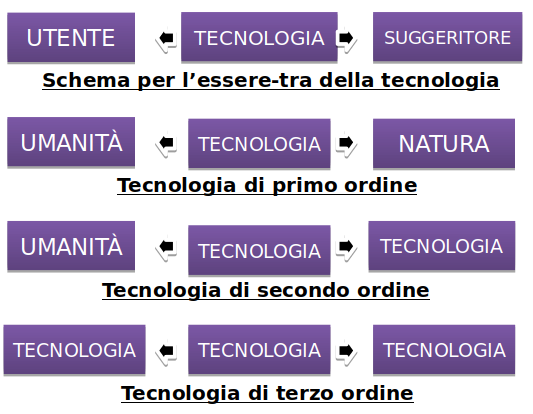
\includegraphics[scale=0.4]{image2.png}
\end{center}
Le tecnologie del terzo ordine sono controllate dall'uomo pur escludendolo (come accade con i dispositivi IoT). \newline

Nel 2011 abbiamo raggiunto per la prima volta un volume di dati dell'ordine dello ZettaByte ($10^{21}$ bytes) e nel 2015 siamo arrivati a $8$ ZettaByte, anche se metà dei dati è stimato essere inutili.
L'Età dello ZettaByte può essere interpretata come il momento di transizioni tra i Big Data ciechi e quelli dotati di vista: nel senso che riesco a dare un senso a questi dati (trovo un pattern).

Legge di Kryder: la capacità di immagazzinamento degli Hard Disk cresce più velocemente della legge di Moore, ma il mondo produce comunque molti più dati di quelli immagazzinabili. \newline
Legge di Nielsen: la velocità di una rete per utenti domestici cresce del $50\%$ l'anno, raddoppiando ogni 21 mesi(meno rispetto alla legge di Moore).

L'innovazione digitale comunque presenta dei rallentamenti, dovuti a:
\begin{itemize}
  \item memoria;
  \item connettività dei dispositivi;
  \item mancanza di standard condivisi: è un tema di grande importanza, si tratta di un primitivismo tecnologico infatti spesso i dati non possono essere elaborati da sistemi diversi da quelli che li hanno prodotti;
  \item dislivello tra innovazione tecnologica e tempi di adattamento delle organizzazioni: DESI (\textit{Digital Economy and Society Index}) è l'indice che mostra il livello di innovazione digitale dei Paesi europei.
  \item albero della conoscenza e sviluppo asincrono: metafora in cui la società è un albero coi rami folti e ingarbugliati, ma con radici (valori etici e culturali) deboli.
\end{itemize}

La quarta rivoluzione è una rivoluzione dell'informazione: l'uomo non è un'entità isolata ma un INFORG: un Organismo Informazionale Interconnesso, che condivide con gli altri uomini un ambiente globale costituito dall'informazione (l'infosfera).
La Sfida della rivoluzione dell'informazione è affermare un nuovo paradigma dell'uomo come animale informazionale al fianco di altri, inserito all'interno dell'infosfera.

L'informazione deve essere considerata un bene di consumo: è un bene non rivale, cioè chiunque ha accesso ai dati può servirsene.
Inoltre non è esclusiva, cioè è più facilmente condivisibile e accessibile e ha un costo marginale tendente allo $0$.
È considerabile quindi un bene pubblico. \newline

Il bitcoin ha introdotto un concetto di scarsità digitale, essendocene una quantità finita.

Gli impatti sulla vita sociale ed economica sono notevoli: il diritto d'uso degli oggetti diventa più importante del diritto di proprietà: ad esempio, il \textit{car sharing} o i servizi di taxi a basso costo riducono il numero di automobili di proprietà.
I beni virtuali, come il software, vengono registrati in bilancio come investimento in conto capitale e non come spese correnti.

Le definizioni dell'INFOSFERA:
\begin{itemize}
  \item a livello minimo, l'infosfera indica l'intero ambiente costituito da tutti gli enti informazionali, le loro proprietà, i loro processi e le reciproche iterazioni (esiste ancora ad un dualismo tra mondo informazionale e mondo analogico);
  \item a livello massimo, l'infosfera è un concetto che può essere utilizzato come sinonimo di realtà (intesa in termini informazionali), è cioè una concezione monistica.
\end{itemize}
Le proprietà dell'Infosfera:
\begin{itemize}
  \item le ICT creano un nuovo ambiente informazionale dove le future generazioni trascorreranno la maggior parte del tempo ``Onlife'' nell'infosfera sempre più sincronizzata, de-localizzata e correlata;
  \item l'infosfera sta riassorbendo l'Habitat ``Naturale'': la soglia tra il mondo analogico, offline, di carbonio e il mondo digitale, online, di silicio tende a sparire;
  \item stiamo passando passando da una metafisica materialistica a informazionale.
  \item l'infosfera tende ad assorbire ogni altro spazio e il mondo offline è destinato a diventare totalmente iterativo grazie all'infosfera.
\end{itemize}
Quindi noi dovremo lavorare a un ecologia dell'infosfera infatti:
\begin{itemize}
  \item il digitale divide e rischia di generare nuove forme di discriminazione tra chi è digitale e chi non lo è;
  \item si creerà un nuovo divario tra società storiche e iperstoriche(per cui l'informazione è un bene);
  \item si ridisegnerà la mappa della società mondiale;
  \item la nuova ecologia è necessaria per evitare le baraccopoli digitali.
\end{itemize}

Per fare questo bisogna essere in grado di essere una gamma di applicazioni che:
\begin{itemize}
  \item migliorano: sono interfacce volte a facilitare l'uso dello strumento (impugnature ergonomiche, interruttori);
  \item aumentano: lo strumento permette un interfacciamento tra due ambienti, quello dell'utente e quello del suggeritore;
  \item apportano trasformazioni radicali: le ICT creano e ricostruiscono realtà che l'utente è in grado di abitare, le loro interfacce sono delle porte d'ingresso per l'utente nell'infosfera.
\end{itemize}

Le tecnologie ICT stanno riontologizzando il mondo: ad esempio con mouse e touch screen.


\section*{Lezione 3 - 12/11/2018}
I social stanno cambiando le nostre identità personali, e questo ci pone delle domande:
\begin{itemize}
  \item chi siamo? (la nostra identità personale)
  \item chi pensiamo di essere? (la nostra concezione di sè)
  \item cosa pensano gli altri su cosa siamo? (la nostra identità sociale)
\end{itemize}

La nostra generazione è inconsapevole di sé, e lavoriamo in tutti i modi per costruire la nostra immagine social in base a quello che gli altri pensano di noi, senza averne però la certezza.

Il risultato è che su Internet siamo la proiezione di chi vorremo essere.
Il nostro sè sociale influisce su ciò che siamo veramente: a causa della condizione sociale alteriamo la nostra identità.
Basta guardare la polarità che si è formata su Internet, ad esempio nel caso delle elezioni.

La domanda è: chi siamo noi e che cosa diventiamo dopo che siamo stati tutto questo tempo nell'infosfera?
Il paradosso della nave di Teseo: continuando a cambiare i pezzi della nave quando marciscomo, alla fine la nave è identica a quella iniziale ma senza neanche un pezzo originale.

L'interfaccia è molto importante per rispondere a certe domande, ad esempio nel caso di un ospedale diventato scuola: è diverso il fine  mentre la struttura è la stessa.
Per rispondere a tale domanda esistono due approcci:
\begin{itemize}
  \item Descartes (Cartesio): ``\textit{Cogito ergo sum}'' (penso quindi sono): le idee sono chiare e distinte. John Locke: l' identità è data dall'unità della coscienza e dalla continuità della memoria.
  \item Teoria narrativa del sè: l'identità è una storia (auto-biografia).
\end{itemize}

Ma, ad esempio, i pazienti di Alzheimer, perdendo spesso rapidamente la memoria, perdono anche la loro identità?
Secondo il primo approccio si tratta di persone diverse mentre per il secondo si tratta della medesima persona in due momenti diversi della propria vita.

Il Sè è dunque un sistema informazione complesso, costituito da attività coscienti e ricordi: noi siamo la nostra informazione.
E le ICT tecnologie che influenzano profondamente il proprio sé.

Concetti informazionali di sé:
\begin{itemize}
  \item una visione dualistica della relazione tra il corpo e la mente;
  \item una forma di monismo basato sullo stato: materiale contro immateriale, come differenti stati dell'informazione (una metafisica informazione): sembra un ritorno alle prime forme della filosofia che studiavano il rapporto tra persona e mondo.
\end{itemize}


Grazie alle ICT nasce l'\textit{e-health}, la sanità che sfrutta i Big Data per migliorare i propri servizi: in futuro la condivisione di dati medici anonimi o anonimizzati sarà fondamentale per la ricerca.
Si parla infatti di \textit{corpo condiviso} perchè il corpo del singolo sarà considerato una fonte di dati per ricerca di pattern su ampia scala; mentre il corpo diventa \textit{trasparente}: nuove tecnologie (smart watch) monitorano costantemente il corpo per migliorare la prevenzione e il benessere individuale.
Si ha quindi una democratizzazione delle informazioni sanitarie e della loro accessibilità, un aumento dei dati generati e una socializzazione delle condizioni di salute.

E-education: \textit{civilizzato}, \textit{acculturato} ed \textit{educato} non sono sinonimi: i primi due si riferiscono a fattori locali, mentre il terzo è più particolare.
Tuttavia nell'infosfera l'\textit{essere educati} è una caratteristica che si sta velocemente de-localizzando e uniformando, in realtà già dalla fine del 1900: l'educazione deriva da una trasmissione di conoscenze, democraticizzate grazie alle ICT.
Le ICT infatti permettono di personalizzare l'esperienza educativa, ad esempio tramite i Massive Open Online Courses disponibili su Internet.

L'\textit{information society} è una neo-società che usa come materia prima l'informazione e produce come prodotto finale altra informazione.
In tale società si pone enfasi sul saper fare (tècne) e non sul sapere teorico (epistème).



\section*{Lezione 4 - 03/12/2018}
La \textit{privacy} cresce di importanza nelle ICT, anche se muta di significato dopo la quarta rivoluzione.
La privacy è una funzione della frizione informazionale: è la resistenza che si oppone alla diffusione libera dell'informazione.
Minore è la frizione informazionale, maggiore è l'accessibilità alle informazioni personali fra gli agenti di una regione.
Minore è il gap informazionale, minore è il livello di privacy che ci si può aspettare.

Con le prime urbanizzazioni il livello di privacy è aumentato notevolmente rispetto alle zone rurali, dove le notizie si diffondevano velocemente all'interno dei paesi.
Ciò che consente alla società urbana lo sviluppo della privacy è l'anonimato: l'identità del singolo individuo spesso non è nota ai più; ma nella società digitale l'anonimato non può essere garantito totalmente.
Con il passare delle generazioni cambia ciò che si vuole tenere nascosto, oggetto di privacy.

Mentre le vecchie ICTs (TV, radio) riducono la frizione informazionale facilitando la diffusione di notizie, le nuove ICT funzionano da entrambe le parti: le tecnologie sono divise in PET (\textit{Privacy Enhancing Tecnology}), che tentano di aumentare la frizione informazionale e di garantrie maggiore qualità e quantità di prodotto, e le PIT (\textit{Privacy Intrudincg Tecnologies}), normate dal GDPR.

Siccome dopo la quarta rivoluzione l'identità dell'individuo è rappresentata dalle proprie informazioni, la mancanza di privacy è un'aggressione contro la persona.
Addirittura si può arrivare al furto di identità, che è uno dei principali attacchi nella società digitale.


sono diversi problemi etici che sorgono dai social network:
L'uso non etico delle informazioni sugli individui ha portato a una serie di problemi, come l'incitamento all'anoressia su blog di moda, giochi suicidi come \textit{BlueWhale} o il caso Target (catena di supermercati statunitensi che ha previsto la gravidanza di una ragazza all'insaputa del padre).

La quarta rivoluzione porta anche cambiamenti a livello politico: entra in crisi lo Stato Nazionale, nato nel 1648 con la pace di Vestfalia (che diede fine alla guerra dei 30 anni e la guerra degli 80 anni), sistema indipendente operante in un contesto nazionale basato sui concetti di:
\begin{itemize}
  \item sovranità: diritto di autodeterminare la propria politica;
  \item equità: le giurisdizioni dei vari Stati Nazionali sono ugualmente importanti;
  \item non interferenza: non sono permessi interventi negli affari interni di altri Paesi.
\end{itemize}
Gli stati nazionali dunque agiscono come agenti indipendenti che possono aumentare tasse entro i loro confini, contrattare debiti come entità legali e difendere i propri confini.
Montesquieu teorizzò la triplice divisione dei poteri dello Stato: legislativo, esecutivo e giudiziario.
Lo Stato è un sistema multi agente organizzato come una rete composta da questi tre aspetti.
Le ICT per uno Stato Nazionale sono uno strumento per esercitare la forza legale, il potere politico e il controllo sociale.

La crisi dello Stato Nazionale inizia col \textit{Washington Consensus} (1989): un insieme di 10 raccomandazioni per fronteggiare crisi economiche.
Le ICT passano da una forma di governo centralizzato a una forma di governo distribuito e di coordinamento internazionale, per gestire crisi di grande complessità internazionale.

Con la conferenza di Bretten Woods (1944) si accentua la crisi dello Stato Nazionale: si formano enti sovranazionali come World Bank, World Trade, IMF (\textit{International Monetary Fund}) con lo scopo di fare da intermediari in problematiche tra i vari Stati Nazionali.
Le 4 conseguenze di ICS, che spiegano il passaggio da una situazione storica a una situazione iperstorica sono:
\begin{itemize}
  \item potere: le ICT democratizzano l'esercizio del potere e ne permettono l'esercizio a entità diverse dallo Stato (multinazionali), facendo sorgere nuove problematiche tra potere informazionale e potere fisico;
  \item geografia: le ICT delocalizzano l'esperienza umana, rendendo irrilevanti i confini statali, creando regione dove prevale l'\textit{onlife}, facendo sorgere nuove tensioni tra la geopolitica globale e lo stato.
  \item organizzazione: le ICT fluidificano la topologia della politica, generando nuove realtà multi-agente non statali (ISIS);
  \item democrazia: le ICT permettono la costruzione di forme di democrazia diretta come opzione complementare, spesso condotta dai mass-media, generando tensione all'interno della democrazia.
\end{itemize}

Internet sta modificando la comunicazione politica: stanno mettendo in pericolo la democrazia?
Le ICT permettono la profilazione economica e politica dei propri utenti ma nello stesso momento diventano necessari per la politica stessa: ``Non potete vincere le elezione stando su Internet, ma perderete sicuramente se non ci siete.''

Dai conflitti storici  armati (i fallimenti della politica) si passa alla \textit{cyberwar} e ai conflitti con i metodi digitali dell'iperstoria.
Infatti le ICT hanno rivoluzionato il modo di scambiare informazioni, rendendo possibili nuove modalità operative.
Le ICT stesse e i Big Data sono delle armi: analizzando rapidamente grosse quantità di dati, l'intelligence militare può prendere decisioni in tempi molto rapidi; mentre le battaglie sono combattute con dispositivi ICT in tempo reale (droni, robot, satelliti, sensori\ldots) o contro bersagli \textit{cyber} mirati, aumentando il potenziale distruttivo degli attacchi.
L'iperstoria modifica anche le forme di terrorismo: si passa dal terrorismo suicida agli attacchi cyber, che possono essere intrapresi sia da interi Paesi sia da piccoli gruppi, facilitando conflitti asimmetrici e facendo sorgere nuove problematiche etiche (sui diritti, i rischi e le responsabilità): l'\textit{information war} ha bisogno di una nuova etica, un regolamento di guerra. \newline

I geologhi concordano nel dare all'epoca attuale il nome di \textit{Antropocene} a causa dell'impatto significativo dell'uomo sull'ecosistema.
La nuova era ha dei costi ambientali  molto alti, se non addirittura insostenibili: l'infosfera mette a rischio la biosfera, quindi bisogna prestare attenzione all'impatto che la tecnologia ha sulla natura.
Per esempio alcuni temi sono il versamento del petrolio in mare o l'esplosione di centrali nucleari (Chernobyl): si stanno sviluppando delle \textit{meta-tecnologie}, cioè  sistemi legali e tecnologie per la sicurezza per minimizzare i danni.
Di fronte a catastrofi ambientali si può reagire in diversi modi:
\begin{itemize}
  \item con la proibizione: un po' troppo radicale, può avere effetti devastanti sui piano di crescita in corso (proibizione nucleare in Italia);
  \item limitazione e riparazione: si tenta di ridurre al minimo i danni grazie alla prevenzione, che però può risultare insufficiente (centrale nucleare di Fukushima);
  \item compensazione: si gestiscono i costi prima del danno tramite assicurazioni o multe, il cui importo però può essere minore del danno causato (dopo un versamento di petrolio in Alaska, la compagnia petrolifera fu multata solo di \$75 milioni ma il danno ammontò a \$2.3 billioni.
\end{itemize}

Le ICT  potrebbero giocare un ruolo molto importante nella crisi ambientale, nonostante l'elevato consumo di elettricità.
È stimato che le emissioni dovute alle ICT aumenteranno di circa 6\% all'anno:  sono sia potenziali \textit{energy savers} sia inquinanti.
Si spera che il beneficio apportato migliori l'ambiente più dei danni causati, e che ci sia abbastanza tempo da recuperare i danni già fatti.


\section*{Lezione 5 - 05/12/2018}
Il mondo sta cambiando dall'analogico al digitale: si mettono in dubbio gli ideali dell'epoca moderna.
L'intelligenza artificiale è stupida e permette alle macchine solamente l'esecuzione di compiti specifici, certo in modo migliore rispetto all'uomo, ma senza capacità cognitiva.
Non c'è più differenza tra online e offline: l'infosfera è un miscuglio di entrambi.
Questi cambiamenti non producono problemi ma sfide: affrontandole bene si avrà una società migliore.
\begin{itemize}
  \def\labelenumi{\arabic{enumi})}
  \item vulnerabilità: il digitale mette a rischio tutti, senza distinzioni, allo stesso modo, ma è il digitale stesso a fornire soluzioni (antivirus);
  \item complessità: non sono note le implicazioni dei singoli cambiamenti (per esempio: come saranno le grandi città in futuro col digitale) nè si possono prevedere;
  \item sostenibilità: bisogna prestare attenzione alle problematiche ambientali, perchè senza un posto da abitare lo sviluppo tecnologico è inutile;
  \item compatibilità con l'offerta di lavoro: lo sviluppo tecnologico deve comunque garantire un salario, le tecnologie devono rendere più efficiente il lavoro, non sostituire l'uomo;
  \item autonomia: è molto importante perché gli accessori comunicano i gusti della persona.
\end{itemize}

La società si divide su 3 piani: o si inventa qualcosa, o si scopre qualcosa o si disegna qualcosa.
Il design deve tenere conto sia dell'ambiente sia del digitale.
L'innovazione deve essere guidata da una strategia secondo delle regole (leggi, come il GDPR, o i diritti umani): queste sono fondamentali, ma senza un'etica non si ha una direzione; inoltre bisogna superare la visione antropocentrica per allargarla all'intero pianeta.

\textit{Dato} e \textit{informazione} sono concetti profondamente diversi.
Il primo infatti rappresenta la mancanza di uniformità tra due elementi (interpretabili) nel mondo reale, tra due stati fisici o tra due simboli; mentre l'informazione si ottiene aggregando un numero sufficientemente grande ($> 0$) di dati ben formati (cioè registrati nel modo corretto secondo regole poste) con un loro significato.
Secondo Floridi, la tecnologia corrente non è in grado di processare informazioni prive di semantica, cioè il significato dei dati è posto solamente dall'uomo.
I computer sono macchine sintattiche che possono processare dati in modo acritico senza interpretarli ma seguendo delle regole (\textit{sintassi}); rimangono però incapaci di apprezzare le caratteristiche semantiche (il significato) delle entità coinvolte e delle loro relazioni.
Il problema fondamentale della robotica infatti è di trovare un modo per far sì che i dati acquistino di significato per una macchina.
Infatti non è noto come l'uomo riesca a processare significati, nonostante l'operazione sia eseguita in modo eccellente: secondo Floridi c'è una soglia semantica tra uomo e macchina che non si riesce a recuperare.
Si parla dunque di Intelligenze Artificiali mettendo in rapporto:
\begin{itemize}
  \item AI forti contro deboli;
  \item in senso ingegneristico contro cognitivo;
  \item in senso produttivo contro ri-produttivo.
\end{itemize}
Cercando di superare le problematiche legate alla semantica dei dati, si sono sviluppate nuove tecnologie, dette le \textit{nuove AI}, tra cui le reti neurali, i sistemi Bayesiani, il Machine Learning e i robot situati.

Visione alternativa è quello di Ray Kurzweil, secondo cui l'invenzione delle AI accelererà bruscamente la crescita tecnologica e cambierà profondamente la civilizzazione come la conosciamo.
Secondo tale ipotesi le AI entreranno in un ciclo di auto-miglioramento che risulterà in una intelligenza superiore a quella umana verso il 2045.

Le AI portano con sé opportunità e rischi per la società, in particolare 4 opportunità principali a cui corrispondono 4 rischi del cattivo uso, del sovrauso e del poco uso:
\begin{center}
	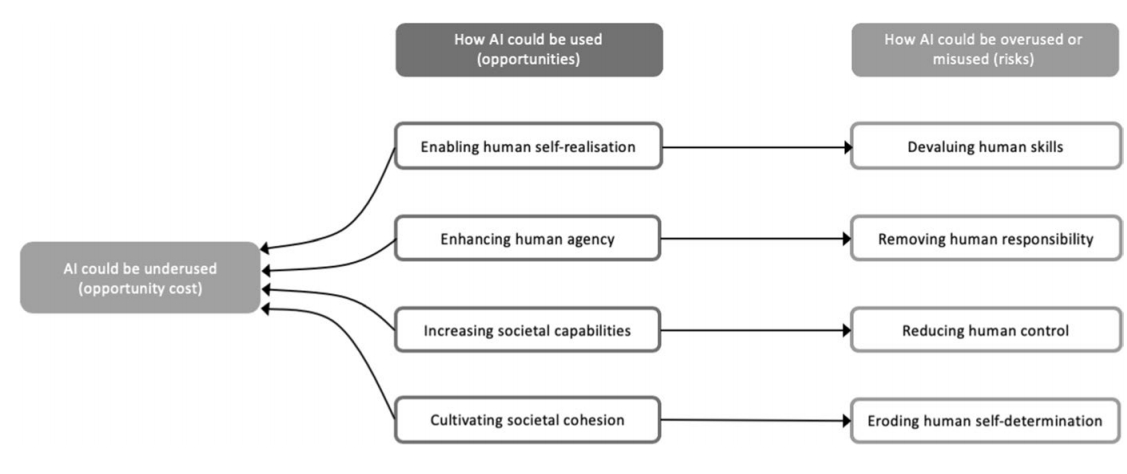
\includegraphics[scale=0.4]{image3.png}
\end{center}

Le 4 opportunità offerte da AI sono:
\begin{itemize}
  \item Chi possiamo diventare: aumentano la propria realizzazione senza devalutare le abilità umane garantendo maggior tempo libero per sè; questo potrebbe però generare una distribuzione non equa di skill e costi-benefici derivanti dall'uso delle AI.
  \item Che cosa possiamo fare: aumentano le possibilità d'agire dell'uomo, senza però rimuovere la responsabilità: permettono di produrre di più e meglio ma la responsabilità umana rimane imprescindibile; si è tentati però di scaricare le proprie responsbilità sulle macchine e di accettare in modo acritico le loro risposte senza accedere alle basi del funzionamento (mentaltià a scatola chiusa, \textit{blackbox}).
  \item che cosa possiamo ottenere: migliorano le capacità sociali senza ridurre il controllo umano, infatti le AI offrono tante possibilità di migliorare la nostra società (nella medicina o logistica) ma il rischio è che, essendo l'uomo fuori dal processo, non ha l'abilità di monitorare a dovere li funzionamento del sistema: è necessario tenere sotto controllo gli sviluppi maggiori e i loro effetti.
  \item Come possiamo interagire: coltivare la coesione umana senza erodere l'autodeterminazione; infatti con i problemi globali sta aumentando il senso di coordinazione complessiva, che può essere trattata solo se tutti i stakeholders cooperano: le AI possono aiutare tanto in questo ambito (ad esempio per il cambiamento climatico) grazie alla loro potenza predittiva, che deve essere al servizio dell'umanità e non toccare la dignità umana.
\end{itemize}

C'è un vantaggio doppio nell'uso etico delle AI: l'etica permette di ottenere tutti i vantaggi dal loro uso, ottenendo nuove opportunità socialmente preferite o accettate, senza però incorrere in errori costosi, prevedendo o mitigando azioni che potrebbero diventare socialmente inaccettabili.

I 5 principi proposti da cui 4 dalla bioetica sono:
\begin{itemize}
  \item la beneficenza: promuovere il benessere, preservare la dignità e sostenere il pianeta;
  \item la non malificenza: privacy, sicurezza e prevenzione di altri danni;
  \item autonomia: il potere decisionale e il libero arbitrio;
  \item la giustizia: promuovere la prosperità e preservando la solidarietà;
  \item la trasparenza e l'esplicabilità: avvia gli altri principi attraverso l'intelligibilità e l'applicabilità, in modo che il sistema sia trasparente a noi.
\end{itemize}


\section*{Lezione 6 - 10/12/2018}
Gli impatti della tecnologia digitale sui modelli del business che hanno caratterizzato il periodo fino al 2015 sono
Le tecnologie digitali si prima del 2015 si sono focalizzate su tematihe come Internet mobile, i Big Data, il Cloud, il crowd sourcing, l'urbanizzazione rapida, lo smart working, i cambiamenti climatici, la volatilità geo-politica, lo sviluppo della classe media e la longevità della vita.
Dal 2015 al 2017 invece ci si è concentrati più su tematiche etiche come la parità di genere, la privacy, nuove etiche e stampanti 3D.
Dal 2018 in poi si hanno la robotica, i trasporti automatici, le AI, e le biotecnologie.

Il periodo di payback\footnote{tempo impiegato prima di ottenere guadagni da un investimento.} nel mondo della robotica sta diminuendo, portando alla luce nuove tematiche: la manodopera robotica ha un alto costo iniziale ma molto inferiore alla manodopera umana nel lungo periodo; per l'imprenditore dunque è un'opportunità sostituire i lavoratori umani con macchinari.
Questo problema è particolarmente sentito nei Paesi in via di sviluppo.
I settori più coinvolti sono i servizi legati alla finanza, alle infrastrutture e alla mobilità (macchine auto-pilote), uffici, amministrazione, produzione, costruzione, estrazione, arte, sport e media; risultano però avvantaggiati altri settori quali informatico, matematico, architettonico e ingegneristico.

Abbiamo che le occupazioni ristrutturate (dove le competenze rimangono sicure, ma la forma del servizio cambia) sono l'insegnante accademico e il fotografo; le occupazioni fuori mercato (obsolete) sono quelle del casellante e del bibliotecario.
Le occupazioni riqualificate (le cui le competenze sono standardizzate ma i consumatori prestano attenzione a come è fornito il valore) sono quelle del muratore e del cameriere al fast-food; mentre le occupazioni durevoli sono quelle del infermiere, idraulico, elettricista.

Il passaggio dall'analogico al digitale ha dei vantaggi e svantaggi: da una parte permette una maggiore ricchezza con minor impiego di lavoro; dall'altra può far perdere lavoro (si veda il caso di Kodak, soppiantata da Instagram) a numerose persone e la ricchezza si può concentrare in mano a pochi individui, facendo crescere il divario economico.
%
% Coloro che sono riusciti a cogliere quest'opportunità e accumulare i giusti assetti:
% \begin{itemize}
	 
% 	\item
% 	Capitali non umani: assetti finanziari, equipaggiamento, proprietà
% 	intellettuali
% 	\item
% 	Capitali umani: educazione, esperienza e abilità.
% \end{itemize}

Quindi questo sviluppo non aiuterà tutti, ma le tecnologie digitali sostituiranno i lavori meno qualificati, mentre il livello di competenze richieste sarà sempre maggiore: si riduce la richiesta per lavori non qualificati, mentre aumenta la richiesta di personale tecnico.
Un'altra questione è l'opinione pubblica pessimista sul futuro nonostante il PIL mondiale non sia mai stato più alto di ora, né l'innovazione tecnologica così rapida: nonostante l'occupazione stia iniziando a scendere, in generale, la produttività continua ad aumentare.

La proposta di Bill Gates di tassare i robots ha suscitato molte polemiche, tra cui quella di Maffè che la definisce un'\textit{idiozia economica} perché ridurebbe l'efficienza produttiva: bisogna affrontare il problema con il Welfare e investendo.
Elon Musk propone una redditto universale, mentre Bentivogli dice di detassare il lavoro umano e introdurre il diritto soggettivo alla formazione per ridurre il gap di competenze.

Marx, nella storia economica, distingue il periodo della manifattura (basato sul lavoro manuale) e il periodo dell'industria moderna (basato sui macchinari): nel pensiero di Marx le macchine assorbono il lavoro.
Nel nostro periodo abbiamo i robot, Internet e le AI, organizzate in modo invisible dal software.
Quest ultimo rappresenta il rischio dell'erosione economica e della divisione del lavoro.
% La didattica tradizionale nel digitale sta diventando data scalabile e condivisibile (ML, AI).
Il software modifica l'erogazione di servizi, privilegiando la gestione del canale rispetto alla qualità del servizio (Uber, Airbnb).
Le tecnologie digitali riducono l'asimmetria tra domanda e offerta portando acquirenti e venditori allo stesso piano; ma si riducono anche le asimmetrie organizzative: si appiattisce la supply chain delle aziende che sfruttano la stessa piattaforma digitale.
Il risultato di tutto questo è la polarizzazione del lavoro: la creatività viene ben pagata mentre le nicchie frammentate marginali riducono la loro paga (Data Scientist vs Badante).
Questa crisi del welfare può essere affrontata redistribuendo il valore generato dai dati: questo tema va oltre la tassazione sui profitti e l'efficienza prodotta dai robot.

Quindi sembra che le nuove tecnologie non aumentino di per sè la povertà, ma al contrario sembra che richiedano nuovi valori: il problema è lo sviluppo delle skill necessarie per stare al passo con l'innovazione, difficilmente ottenibili a causa dell'inefficienza scolastica.
Così  creare nuove tecnologie distrugge i lavori già esistenti più velocemente di di quanto ne crei di nuovi per la lentezza e inefficienza nella gestione del gap di competenze.

La nuova generazione dovrà accelerare la produzione delle opportunità dall'impiego nel settore digitale, e aumentare la velocità di insegnamento dei nuovi capitali umani.
Se si dovesse fallire tutto il sistema perderebbe la sua produttività: la soluzione quindi è aggiornarsi per tutta la vita per stare al passo con la tecnologia.

Per le vecchie generazioni abbiamo due scenari:
\begin{itemize}
  \item una sorta di ``piano Marshall''\footnote{Piano di sviluppo economico favorito da prestiti USA in Europa per rilanciare gli investimenti imprenditoriali dopo la Seconda Guerra Mondiale.} per rigenerare le skill;
  \item riconvertire le skill non produttive per i servizi sociali, in un nuovo sistema di auto sostenimento basato sui sussidi.
\end{itemize}


\section*{Lezione 7 - 12/12/2018}
Le tecnologie digitali stanno modificando il mercato: si passa da una gestione di tipo verticale (concentrata cioè su un unico settore) ad ecosistemi di soggetti appartenenti a più ambiti, alcuni anche nuovi, che entrano in contatto grazie alle ICT.
Si parla di aziende \textit{piattaforma} che mettono a disposizione i loro dati a terzi, garantendosi così un guadagno, per fini una volta impensabili.
Il digitale dunque mette in comunicazione aziende diverse di ambiti diversi e di dimensioni diverse: sono industrie orizzontali.
Un esempio è e015 nel settore software della Regione Lombardia.

Le tre leggi di robotica di Asimov sono:
\begin{enumerate}
  \def\labelenumi{\arabic{enumi}.}
  \item Un robot non può recar danno a un essere umano né può permettere che, a causa del proprio mancato intervento, un essere umano riceva danno.
  \item Un robot deve obbedire agli ordini impartiti dagli esseri umani, purché tali ordini non contravvengano alla Prima Legge.
  \item Un robot deve proteggere la propria esistenza, purché questa autodifesa non contrasti con la Prima o con la Seconda Legge.
  %fonte: https://it.wikipedia.org/wiki/Tre_leggi_della_robotica
\end{enumerate}

Visto l'aumento dell'aspettativa della vita sopratutto in Italia e in Giappone, la mancanza di badanti ha creato una nuova opportunità per l'industria: la creazione di robot badanti (Toyota e Honda).
Ma i robot possono prendersi cura degli umani?
Sicuramente possono aiutare nella mobilità e in altre attività quotidiane ma non sono in grado di formare relazioni emotive, sono capaci sono di sentire i dialoghi ma senza capire.
Sicuramente da un punto di vista economico potrebbe rappresentare una forte crescita del mercato dei robot.
Oggi come oggi il 70\% dei robot viene venduto in Cina, Giappone, USA, Sud Corea e Germania: mentre in USA e Germania si vendono di più i robot di alto valore, sopratutto in ambito medico, in Sud Corea e Cina si vendono i robot economici per uso commerciale.
Il Giappone è il mercato con più richiesta mentre la Cina è il mercato in maggior crescita.
Questi robot nel futuro si uniranno in un unico ecosistema per accelerare maggiormente la crescita.

C'è anche la questione dell'accettare un essere robotico, dovuto all'immagine costruita in Occidente secondo cui i robot sono una minaccia per l'umanità, mentre in altre culture, come la religione antica Shinto, si crede che anche gli oggetti non animati siano vivi.

I robot sostituiranno gli umano nel mondo del lavoro in 2 fasi: la prima è quella primordiale dove inizieranno a fare i lavori più semplici mentre nella seconda fase assumeranno i lavori più complessi.

Sono 3 le chiavi che rendono ciò possibile:

Questo sarà possibile grazie all'analisi matematica dei problemi e la formulazione di algoritmi per risolverli e dare un senso a contesti nuovi, allo sviluppo di immense fonti condivise di dati da processare per esercitare gli algoritmi e allo sviluppo dei materiali di costruzione, che permetteranno robot sempre più sofisticati.

Già i robot chirurgici giocano un ruolo abbastanza importate nelle sale operatorie dove si ha tolleranza zero di errori: circa 1 milione di pazienti Americani si sono sottoposti a interventi chirurgici effettuati da robot.
Si hanno per esmepio i micro robot, che possono essere inseriti nel corpo umano per rilasciare radiazioni nella cura contro il cancro, oppure dei robot che assistono nelle lezioni.

Gli umani hanno un capex (\textit{capital expenditure}, costo iniziale) basso ma un alto opex (\textit{operation expenditure}, costo operativi), i robot hanno i costi invertiti: se il capex dei robot scende e l'opex degli umani continua ad aumentare (come accade), conviene investire in robot, che taglieranno diversi posti di lavoro ma nel lungo periodo creeranno nuove realtà lavorative e un immenso valore.
I benefici vanno però all'intera società siccome si possono redistribuire.
I Paesi che sono posizionati in modo migliori sono proprio Sud Corea, Giappone e Germania, visto che stanno sviluppando il settore dei robot per esportarli, dando lavoro ai proproi ingegneri e alle proprie industrie di manifattura.
L'industria cinese ha sfruttato sempre il basso costo della manodopera, ma ora è in rischio e ha due possibili scelte: concentrasi nello sviluppo delle industrie del futuro oppure mantenere la manodopera sempre bassa forzando la sua policy dell'urbanizzazione.

Un altro ambito in sviluppo è la genomica, che si basa sulla decodifica del genoma umano.
Il prezzo di tale mappatura sta scendendo molto velocemente creando nuovi lavori: diagnosi, terapie e medicinali basati sulla genetica, un mercato con un valore di \$11 miliardi nel 2013 e in forte crescita.
Decodificare il genoma significa studiare il DNA in Gigabytes di Big Data, in modo da studiare le proteine che si stanno mutando per diagnosticare, ad esempio, il cancro e studiare quali medicinali potrebbero fermare la mutazione.
Grazie alle tecnologie si sta tentando di ridurre il gap tra le terapie mirate ad una specifica patologia e quelle più generiche.

Ci sono sfide anche nei settori neurologici e psichiatrici, per capire il funzionamento del cervello e trattare le malattie mentali: oggi i trattamenti si basano ancora su studi e sistemi molto vecchi (ad esempio gli antidepressivi pur aggiustando gli equilibri chimici hanno effetti collaterali molto seri).
La genomica può essere di grande aiuto in questo ambito, cercando pattern nel ruolo dei geni.
% Si potrebbero prevenire i suicidi, che sono forse dovute alla produzione di alcune proteine presenti nel corpo di tante persone che si sono suicidate.

Ma vi sono diverse implicazioni etiche: ad esempio, l'eugenetica per creare dei bambini perfetti.
La genomica potrebbe addirittura aumentare il divario socio-economica già persistente, ma potrebbe forse portare anche in vita animali estinti.

Uno dei progetti più importanti è il Human Genome Project degli USA, ma la Cina sta investendo tantissimo in questo ambito e sta recuperando; un cattivo esempio è la Russia con la sua eredità Lysenko (la genemica diventa una pseudoscienza borghese).
Comunque grazie alle nuove tecnologie mobili si possono diffondere le cure mediche nelle zone remote e rurali, inizialmente solo per i più ricchi per poi ridurre i costi permettendo anche al resto della popolazione di usufruirne.

Un altro settore è quello della cybersecurity che è stimato essere un mercato con un valore di 175miliardi di dollari, e anche questo sta crescendo.
La maggior parte degli attacchi informatici sono:
\begin{itemize}
  \item sulla confidenzialità della rete, per rubare o rilasciare informazioni (di solito riguardanti le carte di credito) in modo illecito (Target 2013, Nord Corea contro la Sony nel 2014\ldots{})
  \item colpire la disponibilità di una rete, cercando di mettere giù il sistema bombardandolo con un numero massiccio di informazioni, (Estonia nel 2007, Nord Corea-Sony);
  \item turbando l'integrità di una rete, cercando di cambiare o distruggere il codice del sistema o danneggiare le infrastrutture.
  \item attacchi immischiati: il phishing trasforma la confidenzialità in integrità, mentre i ransomware richiedono un ricatto per sbloccare il PC;
  \item gli attacchi contro dispositivi IoT, reti di oggetti con il potenziale di trasmettere e ricevere i dati.
\end{itemize}

La crescita dell'Internet of Things ha 4 ragioni principali:
\begin{itemize}
  \item numero di autovetture connesse a Internet;
  \item numero di dispositivi smart vestibili;
  \item domotica;
  \item manifattura smart.
\end{itemize}


\section*{Lezione 8 -- 19/12/2018}
Oggi giorno il telefono è la banca, ad. Esempio Ebay, Paypal e ApplePay, Google Wallet. Quindi il nostro denaro sarà codificato e spezzato in 0 e 1 e avvolto con potenti tool di encryption. Il mobile payment va oltre le carte di credito tagliando intermediazioni e riducendo la frizione del mercato. Inoltre rifocalizzando l’economia verso l’innovazione dal basso e valorizzano le attività imprenditoriali, contribuiscono alla lotta contro ineguaglianza causata da queste innovazioni e consentono di raggiungere le comunità più isolate e i mercati emergenti nell’economia globale.

Ad esempio in Africa l’utilizzo di MobilePay è oltre 80\% e non ci sono restrizioni legali sui Mobile payment, un esempio è M-Pesa in Kenya:
\begin{itemize}
	\item E’ un’economia virtuale non bancaria.
	\item Permette Trasferimenti di denaro, mutui e risparmi.
	\item Facilita il pagamento dei salari e bollette e il pagamento internazionale.
	\item Con dei contratti facilita la rimessa dei soldi dei lavoratori emigrati.
\end{itemize}
E questo permette ai stati in via di sviluppo di:
\begin{itemize}
	\item Bypassare la fase di sviluppo delle banche
	\item Elimino i costi del intermediario finanziario
	\item Combattere la corruzione
\end{itemize}
La fiducia è una assunzione per la codificazione del denaro, mercato e pagamento. Ad esempio nel caso di Ebay: le transazioni sono basate sono un rapporto di fiducia tra il venditore e cliente, non cieco poiché è gestito da un sistema di rating e algoritmi monitorato dai owner della piattaforma. 

Il prossimo passo è la Sharing Economy: basato sulla combinazione della tecnologia delle piattaforme impacchettate come applicazioni per creare un mercato peer2peer. Connettono persone con un bisogno specifico con il servizio Ad esempio Uber e AirBnB. 

Le implicazioni della sharing economy:
\begin{itemize}
	\item Dispersione: Le transazioni sono spinte verso le persone locali
	\item Concentrazione: Le transazioni sono ridirette verso le piattaforme, che spesso si trovano in California o Cina.
	\item Rinforzano le classi media, fornendo a loro ulteriori guadagni.
	\item Creano nuove forme di lavoro con più flessibilità ma meno protetti dai diritti.
	\item Dobbiamo migliorare la rete di sicurezza e la sfida di creare e finanziare un nuovo welfare.
	\item Norme incorporate nel mercato codificato e nuovi algoritmi cambieranno le norme già esistenti.
\end{itemize} 

%%%%%%%%%%%%%%%%%%%%%%%%%%%%%
%%%%%%%%%%%%%%%%%%
%%%%%%
%BLOCKCHAIN%
%%%%%%
%%%%%%%%%%%%%%%%%%
%%%%%%%%%%%%%%%%%%%%%%%%%%%%%

Blockchain è una macchina per creare fiducia nata 10 anni fa il 31 ottobre 2008, è un grande registro (ledger) su cui le transazioni sono loggate, è un database che mostra ciò che possiede chiunque in un qualunque dato momento.
Un suo esempio è Bitcoin, infatti ciascuna transazione di esse è registrata sulla blockchain. 
Siccome la blockchain è pubblica e decentralizzata questo registro è distribuito su ciascun utente della blockchain. 
Ciò riduce anche la possibilità di frodi e fa diventare la blockchain un ente indipendente
Per assicurare le che milioni di copie del registro siano tutte aggiornate, Bitcoin è fatto in modo da:
\begin{itemize}
	\item Aggiornare il registro a intervalli regolari.
	\item Aggregare ciascuna transazione condotta con la chiave privata sulla rete dall’ultimo aggiornamento.
	\item Cumularli in un grande blocco che poi si aggiunge al registro creando la blockchain
	\item Per aggiungere la chiave al registro, i computer nella rete devono risolvere un algoritmo randomizzato e complesso.
	\item Una volta risolto il computer trova la soluzione e la invia insieme al block delle transazione da essere aggiunto alla chain, dicendo all’intera rete quando aggiornare.
\end{itemize}
La blockchain permette di decentralizzare le transazioni togliendo la figura dell’intermediario.
Vista la sicurezza potrebbe diventare un protocollo per le transazione sicure, diventando una piattaforma su cui si costruiscono nuove innovazioni. 
La blockchain potrebbe rappresentare un soluzione a basso prezzo per le transazione che richiedono un intermediario per fare da garante. Ma allo stesso momento sfida il ruolo della pubblica amministrazione nel suo ruolo da garante.
Non da confondere il Bitcoin è solo una applicazione della blockchain che è la tecnologia. 

Siamo in una fase di transizione epocale, non solo per il cambiamento dal modello economico centralizzato a quello decentralizzato, ma anche nel nostro ruolo nella società. 
Bisogna capire fino a che punto ci possiamo assumere le responsabilità delle nostre azioni, ad esempio se perdessi il mio wallet digitale o la chiave privata, perderei tutti i soldi su di esso. 
Potrebbe avere ragione Fromm che dice "L'uomo ha paura della libertà".

Anche le strutture centralizzate si stanno muovendo verso l'integrazione di strutture decentralizzate, un esempio è la Blockchain Island di Malta. Malta è la prima Blockchain Island.

Altri ambiti che la blockchain può rivoluzionare sono quelli dei Social Media e pubblicità, decentralizzandolo evitiamo i problemi riguardante la raccolta e gestione dei nostri dati, es. Kin contro FaceBook e indorse contro LinkedIn.

I Big Data sono costituiti da n dati per cui n che tende a prendere tutti i dati (può essere considerata una definizione sintetica), le applicazioni sono tantissime tra le quali:
\begin{itemize}[noitemsep]
	\item Traduzione macchina
	\begin{itemize}[noitemsep]
		\item Pro: Permette a gente comune di tradurre i testi velocemente, permette una globalizzazione veloce, Inglese non ci servirà come lingua principale, ecc.
		\item Contro: Perdita di lavoro degli interpreti, rischio di frodi a causa delle voci clonate.
	\end{itemize}
	\item Riduzione della fame mondiale che affligge circa 800 milioni di persone:
	\begin{itemize}[noitemsep]
		\item Usando i Big Data applicati all’agricoltura possiamo sfamare le persone.
		\item Agricoltura da precisione, che viene dopo la rivoluzione Verde (età industriale) preceduta dalla rivoluzione agricola, porta l’agricoltura nell’età digitale raccogliendo e valutando dati raccolti dai sensori, GPS e modelli meteo per migliorare l’agricoltura fornendo istruzione precise agli agricoltori. 
		\item L’algoritmo rimpiazza l’istinto.
	\end{itemize}
	\item Fintech è un esempio nel campo bancario che sfruttando algoritmi permette di migliorare le operazioni e sviluppo dei prodotti.
	\begin{itemize}[noitemsep]
		\item Una banca è un registro su quanti soldi la banca deve alle persone e quanto le persone debbano alla banca. Ciò lo rende qualcosa di più rispetto a semplici dati.
		\item La banca si sta dirigendo nel verso di un sistema bancario tecnologico.
	\end{itemize}
\end{itemize}
I Big Data aumentano ma con loro aumentano anche i problemi collegati alla Privacy:
\begin{itemize}
	\item I dati vengono raccolti dai servizi di intelligence, es. telefono, webcam.
	\item Ciò ha fatto sorgere una serie di regolamenti in UE riguardante la privacy (GDPR).
	\item Ormai siamo in un punto dove non possiamo fermare la raccolta dei dati quindi ci dobbiamo concentrare sul loro utilizzo lecito.
\end{itemize}
Inoltre ci rende più schiavi degli algoritmi, trasformandoci in macchine togliendo ci l’autonomia e l’istinto umano, ciò potrebbe essere anche vantaggioso ma il costo può essere alto. Infine, il problema è alla fine a chi appartengono questi dati? (A me o a Facebook).

La competitività di un paese, regione o territorio delle industrie del futuro è basato sul controllo dei dati e la potenza di calcolo oppure dipende dalle industrie verticali? Dove le industrie verticali hanno una conoscenza profonda di una singola industria.
 
C’è una scuola di pensiero che dice l’economia del futuro sarà concentrata sul controllo dei Big Data e il Big Data assorbirà ogni altra forma di industrie. Mentre l’altra scuola dice il contrario, che i Big Data saranno solo un tool di supporto ad esempio nel caso di genomica. Il Big Data richiede solo la giusta combinazione di algoritmi e gli esperti del dominio per generare una ricchezza a livello mondiale, uno degli esempi sono le industrie 4.0.

\section*{Lezione Bellini 1 - 14/11/2018}
Il digitale sta trasformando ciò che siamo: da individui diventiamo utenti social; anche la rete sociale passa da analogica (compota dalle persone che ci circondano) a digitale (social network).
Cambia il modo di essere cittadini, si parla sempre di più di \textit{e-cittadini}.
Cambia anche il modo di comprare e vendere: il cliente diventa digitale.
In questo periodo diverse tecnologie si stanno incrociando portando a un'economia informazionale e a una società iperconnessa.

Definizione di tecnologia: dal greco $\tau\epsilon\kappa\nu\eta$ (tècne), studio di un arte o mestiere, conoscienza pratica proveniente dallo studio di una scoperta scientifica (o una procedura produttiva).
Le rivoluzioni tencologiche (informazionali) più recenti sono quella delle ICT (1980) e IoT (\textit{Internet of Things}, 2010). \newline
Definizione di società: insieme di individui soggetti a regole comuni, definite attraverso un sistema ordinato di relazioni politiche, economiche, legali, morali e culturali (semplificando, è una rete sociale).

È la tecnologia ad avere un effetto sulla società oppure è la società che determina la tecnologia?
Negli anni '20 si pensava al determinismo tecnologico: la società dipendeva dalla tecnologia.
Ma negli anni seguiti la teoria fu criticata, arrivando a Castells che replica che né la tecnologia determina la società né il viceversa: la tecnologia è la società, nel senso che non è possibile capire una senza l'altra.
Tanto è vero che lo Stato-società può accelerare o rallentare lo sviluppo tecnologico: ad esempio la Cina dopo il XV secolo l'harallentato, mentre il Giappone dopo il 1860 l'ha accelerato; allo stesso momento la tecnologia può cambiare radicalmente una società.

Questa età dell'informazione è caratterizzato dall'unione di microelettronica, ingegneria genetica, elaborazione dei dati, optoelettronica e telecomunicazione.
La conoscenza perde la sua centralità a favore delle nuove tecnologie.
Dopo la Seconda Guerra Mondiale (1939-45), si ebbero due eventi importanti: la prima commercializzazione di un calcolatore programmabile (1951) e l'invenzione dei transistor (1951); queste due invenzioni segnano l'inizio della Rivoluzione Informatica, divisa allora in tre macro-campi: microelettronica, IT e telecomunicazioni.
Alla fine degli anni '90 si ebbe l'invenzione di Internet, altra invenzione rivoluzionaria: si entra così in un'era d'informazione.
Le informazioni sono solamente un materiale grezzo: queste nuove tecnologie ne ricavano di nuove basandosi sull'informazione stessa.
Un altro fattore importante è la diffusione delle tecnologie informatiche: il fattore più importante nel progresso tecnologico è la loro costante convergenza in un sistema sempre più sofisticato e integrato.

Alla fine del XX secolo i due modi dominanti di produzione, influenzati dalle ideologie politiche polarizzate, sono:
\begin{itemize}
  \item Statismo: caratterizzato da una forte e influente presenza dello Stato nel sistema socio-economico; il controllo del surplus è esterno alla sfera economica e appartiene al Governo;
  \item Capitalismo: caratterizzato da una separazione tra il produttore e i mezzi di produzione; il surplus è organizzato e distribuito all'interno della società.
\end{itemize}
I sistemi di sviluppo con cui si passa dalle materie prime al prodotto finito invece sono:
\begin{itemize}
  \item industrialismo;
  \item informazionalismo: è un evoluzione dell'industrialismo.
\end{itemize}
L'informazionalismo sta rimpiazzando l'industrialismo come paradigma tecnologico dominante, ma quest ultimo non sta sparendo: rimane incorporato nell'informazionalismo, essendone la fase precedente, perchè l'informazionalismo presuppone l'industrialismo per la produzione dell'energia e altre tecnologie.

Il fattore storico principale che ha determinato quest'accelerazione, diffusione e sviluppo dell'IT è la ristrutturazione ed evoluzione del capitalismo in \textit{capitalismo informazionale}.
Le proprietà di quest'evoluzione sono:
\begin{itemize}
  \item un'economia globalizzata;
  \item una maggiore flessibilità nel gestire, decentralizzare e interconnettere compagnie sia internamente che esternamente;
  \item un cambiamento dell'organizzazione lavorativa e una diversificazione delle relazioni;
  \item il declino dell'influenza dei sindacati;
  \item un aumento della forza lavoro femminile;
  \item la liberazione del mercato dal parte dello Stato.
\end{itemize}
  

\section*{Lezione Bellini 2 - 29/11/2018}
Le compagnie più grandi oggi hanno in comune modelli di business basati sulle piattaforme: grazie a queste, le multinazionali scambiano valore tra produttori esterni e consumatori, non più in forma analogica (per esempio tramite i negozi), ma in modo digitale su Internet.

Su una piattaforma i 4 attori principali sono: i produttori, i consumatori, i providers e i proprietari della piattaforma.
\begin{center}
	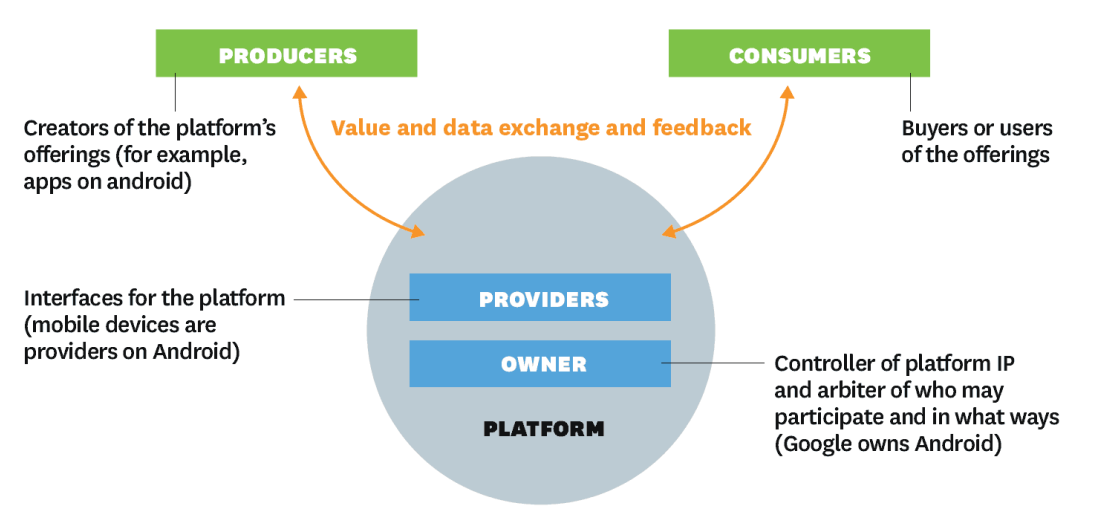
\includegraphics[scale=0.4]{image4.png}
\end{center}

Nel business delle piattaforme non si ha un asset: il valore deriva dagli utenti connessi e dalla comunità formatasi attorno alla piattaforma.
Questi modelli sono aperti e permettono la partecipazione: il vantaggio di questo modello è che le imprese possono definire le proprie regole ed architetture.
Le piattaforme scalano molto rapidamente e si basano sugli effetti del network: l'economia di scala è \textit{demand-side} (dipende cioè dal numero di utenti che usano il servizio) e non \textit{supply-side} come nel modello tradizionale.

Quando parliamo di effetto network abbiamo due categorie:
\begin{itemize}
  \item same-side (diretto): da produttore (o consumatore) a un altro produttore (o altro consumatore), il valore cambia al variare del numero di utenti dallo stesso lato (Whatsapp);
  \item cross-side (indiretto): da produttore a consumatore (o viceversa), il valore cambia al variare di una comunità rispetto all'altra (Trip Advisor, Uber).
\end{itemize}
\begin{center}
	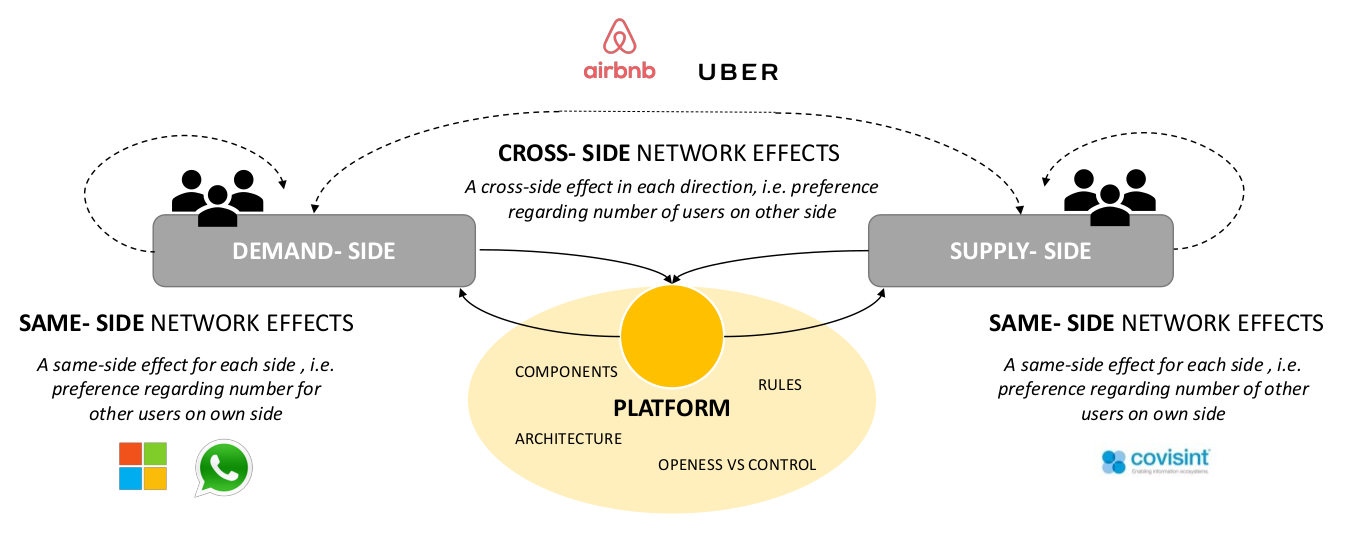
\includegraphics[scale=0.35]{image5.png}
\end{center}
Gli effetti possono essere sia positivi che negativi:
\begin{center}
	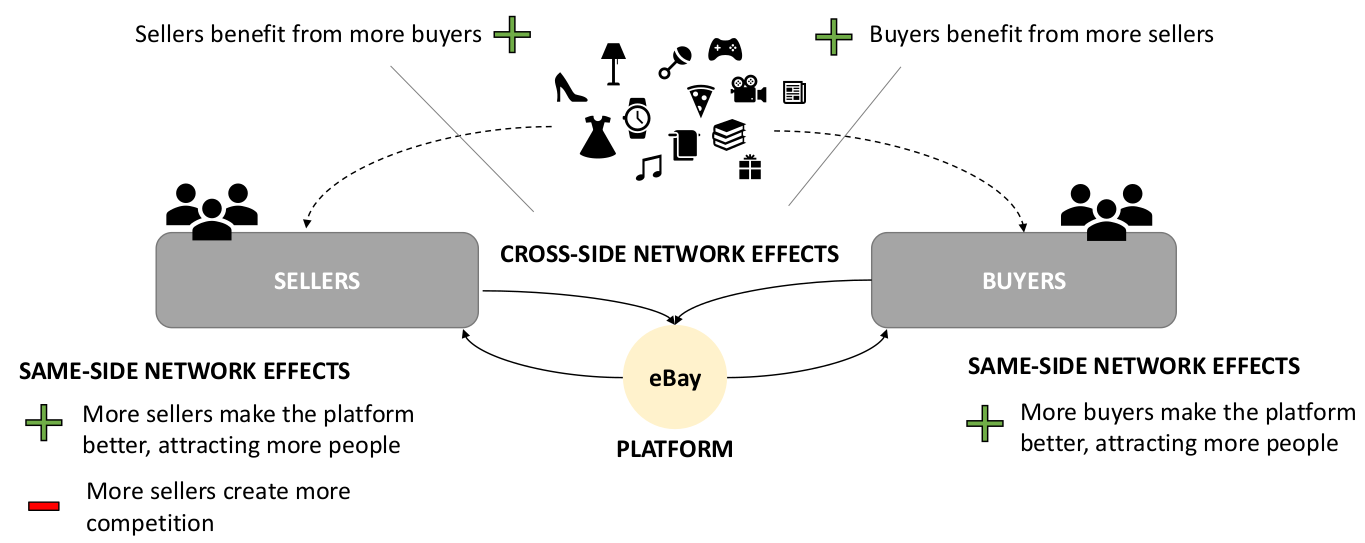
\includegraphics[scale=0.35]{image6.png}
\end{center}

Caratteristica cruciale che permette il successo a questi modelli è l'architettura, dovuta alla modularità: il sistema di business è diviso in un insieme di unità funzionanti, che compongono un'applicazione più grande.
Quindi una piattaforma, in termini di architetture, è fatta di 3 elementi:
\begin{itemize}[noitemsep]
  \item un insieme di componenti principali con un design stabile;
  \item un insieme di componenti complementari;
  \item un insieme di interfacce fisse che permettono inter-operabilità.
\end{itemize}
La modularità permette l'evoluzione e generazione di un ecosistema digitale.

Un altro punto fondamentale è il trade-off tra apertura e controllo su tali sistemi: troppa apertura può portare alla frammentazione e alla perdita di valore mentre troppo controllo può inibire l'innovazione; quindi gli owner delle piattaforme devono adottare un compromesso adeguato.

Questo trade-off tra controllo e generatività può essere espresso attraverso la governace delle piattaforme; i 4 punti fondamentali di questa governance sono:
\begin{itemize}[noitemsep]
  \item la legge;
  \item le norme;
  \item l'architettura;
  \item il mercato.
\end{itemize}

Anche la self-governance è molto importante (e spesso efficace) per le piattaforme.
Sono ancora pochi i settori dell'economia rivoluzionati da queste piattaforme, e hanno un potenziale altissimo.
Sempre più settori si stanno avvicinando a questo approccio: questi settori sono solitamente pieni di informazioni, molto frammentati e hanno un'asimmetria informazionale estrema; mentre i settori che sono pesantemente regolamentati e hanno un costo di fallimento molto alto non verranno modificati tantissimo da questo modello di piattaforma.

L'informazione è costosa da produrre ma la sua riproduzione è quasi gratuita: il costo fisso della produzione è un \textit{sunk cost} non recuperabile una vota fermata la produzione.
Il valore dell'informazione è posto dal consumatore e non dal costo di produzione, ma le persone valorizzano l'informazione in modo diverso; si ha dunque un paradigma diverso rispetto al mercato di prodotto.
Esistono tre metodologie principali di pricing:
\begin{itemize}
\item personalized pricing: il prezzo è ottimizzato in base a quanto ciascun cliente è disposto a pagare;
\item versioning: si offre una linea di prodotto per far sì che sia l'utente a decidere la versione più appropriata;
\item group pricing: si offre un prezzo diverso per gruppi di consumatori (sconto studenti, over 60\ldots)
\end{itemize}

Un bene \textit{esperienzale} è un bene che deve essere consumato dall'utente per valorizzarlo (ad esempio un film); la maggior parte dei nuovi prodotti sono beni esperienzali, e l'informazione non fa eccezione.
Per un cliente comprare informazioni prima di conoscerne il contenuto può essere un problema, ma si adottano diverse strategie, come offrire un'anteprima o basarsi sulla reputazione del venditore.
Questo problema rimane uno dei più grossi dell'Information Age; inoltre il problema non rimane più l'accesso all'informazione bensì il suo sovraccarico.
L'interfaccia che permette di salvare, cercare, recuperare, copiare, filtrare, manipolare, vedere, trasmettere e ricevere l'informazione è la tecnologia.

\section*{Lezione Batini - 21/11/2018}
La parola ``dato'' deriva dal latino \textit{datum}, ciò che è stato dato: i dati rappresentano il mondo che è passato almeno storicamente.
Astraendo il concetto di dato si passa all'informazione e infine alla conscenza.

Ad esempio misurando la temperatura corporea con un termometro, la temperatura è un dato; il dato è una codifica grezza dei fenomeni del mondo, e da cui si posso trarre informazioni.
Trarre informazioni però dipende dalla conoscenza pregressa: abbiamo che il dato 37.5 (la temperatura) diventa informazione se noi sappiamo cos'è la temperatura corporea e come si misura; in questo caso abbiamo che l'informazione è: ``La temperatura corporea è pari a 37.5 $^o$C'' e con la conoscenza pregressa possiamo concludere di avere una febbre leggera, accrescendo quindi la nostra conoscenza.

La produzione dei dati, in generale, avviene osservando la realtà attraverso un compleso processo di rappresentazione al fine di produrre un risultato (o una rappresentazione), che può variare in base al soggetto rappresentante o all'obiettivo ultimo.
Ad esempio guardando un tramonto si può avere una foto, una poesia o un post sui social.

Il passaggio dai piccoli dati ai Big Data avviene principalmente in 3 direzioni (con metafora del cubo o della sfera in espansione):
\begin{itemize}[noitemsep]
  \item l'ampiezza della realtà osservata: ad esempio grazie ai satelliti è possibile vedere le cose da molto più in alto con molta più precisione;
  \item la profondità nella conoscenza della realtà osservata: ad esempio i sensori nelle ruote di una macchina che le rendono ``intelligenti'';
  \item il tempo: si può studiare l'evoluzione nel tempo di tante cose con scale completamente diverse: ad esempio il progresso di una città in 	mesi, oppure lo spostamento dei voli in secondi.
\end{itemize}
Le tecnologie (in blu) che alimentano i Big Data e le loro dipendenze possono essere schematizzate:
\begin{center}
	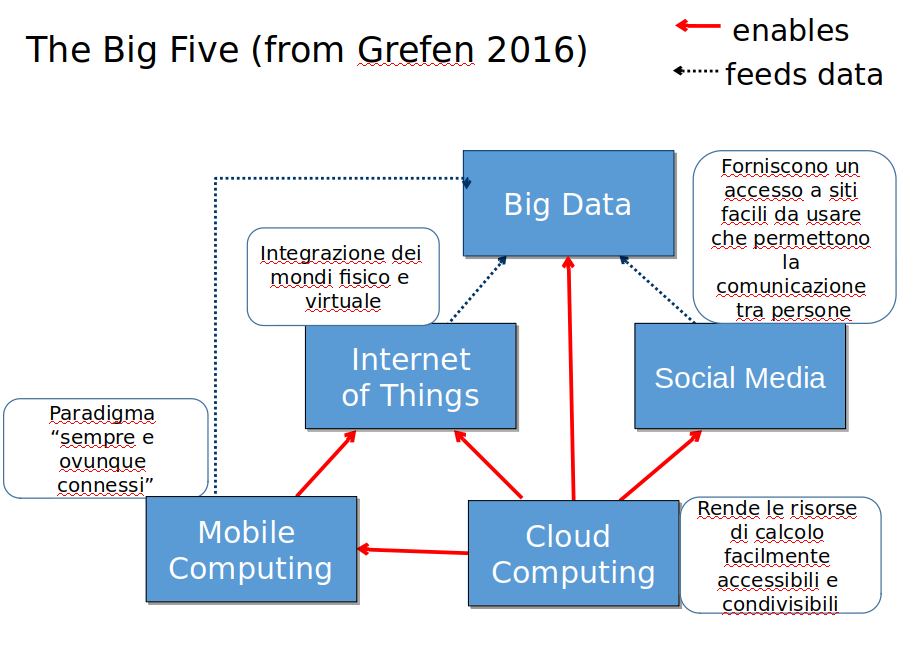
\includegraphics[scale=0.39]{image7.png}
\end{center}

Ciclo di vita dell'informazione:
\begin{itemize}
  \item formulazione del problema: devo capire a cosa mi possono servire i dati.
  \item scelta delle fonti;
  \item gestione (o preparazione)
    \begin{itemize}
      \item valutazione e miglioramento della qualità;
      \item trasformazione;
      \item arricchimento semantico;
      \item integrazione;
      \item eliminazione dei dati non rivelanti;
    \end{itemize}
  \item visualizzazione esplorativa
  \item analisi
    \begin{itemize}
      \item statistica classica;
      \item Machine Learning;
      \item validazione della tecnica;
    \end{itemize}
  \item visualizzazione dei risultati.
\end{itemize}

Secondo il \textit{World Economic Forum} nel 2013, tra le minacce più grandi per l'umanità si sono aggiunte le frodi di massa e i furti dei dati, i cyberattacchi e la disinformazione digitale.
Sempre più persone usano tecnologie che costano sempre di meno e con cui riescono a migliorare la produttività.
Ad esempio l'intelligence si aiuta con computer per le analisi e machine learning, che avranno una potenza migliore in futuro.
Le AI possono essere usate non solo per analizzare i dati ma anche per produrli (si veda il caso di nuove facce generate da Nvidia oppure gli ultimi giocatori robot di Go): questa generazione di AI sarà la causa della scomparsa della fiducia sociale, poiché le prove, prima considerate affidabili, non lo saranno più (un caso attuale è deepfake).

Il passaggio dall'analogico al digitale può generare ambiguità, ad esempio con la digitalizzazione del catasto si pensava di aumentare la trasparenza e la tracciabilità, ma i contadini non si sono rilevati in grado di utilizzare i sistemi informatici rendendo necessario l'intervento di un intermediario.

Il valore dei dati è un concetto molto ampio: si possono scoprire gli evasori unendo vari dati riguardo a una persona (usando ML), oggi divisi in più dataset; oppure si possono prevedere i livelli di inquinamento: BreezoMeter, una start-up israeliana, sfruttando combinazioni e integrazioni di dati e ipotesi provenienti da fonti diverse, produce delle heatmap da cui si possono fare previsioni

La sostituzione dell'uomo con le macchine non è simmetrica: data la dimensione delle masse, necessariamente vengono sfruttate procedure automatiche, e solo chi sfrutta le masse è in una  posizione di privilegio.
Si hanno però esempi sociali dell'uso dei dati.
Per esempio in Uganda i dati riguardanti la health-care sono stati resi pubblici e ciò ha ridotto la mortalità dei bambini con meno di 5 anni di un
terzo, senza procedere in analisi di alcun modo.
\end{document}
